To estimate a limit on the isomerization, we consider the above reaction \cref{r: X+COH->HCO,r: X+COH->XH}, where \ce{X = ^{15}N2} in the context that we can only determine the abundance of \ce{[HCO]+} and \ce{^{15}N2H+}. As a function of pressure, we cannot see reaction \ref{r: X+COH->HCO}, but if it does contribute, we should see a discrepancy in the total rate constant, which we estimate to be Langevin: $k_L = 8.0 \times 10^{-10}$. The functional form is as follows:

%\begin{align}
%    \eta & = C\left(1-e^{-k_\ref{r: X+COH->XH} \rho \tau}\right) \\
%    k_\ref{r: X+COH->XH} & = \frac{\ln\left(C-\frac{^{15}N_2H^+}{^{15}N_2H^+ + [HCO]^+}\right)}{\rho \tau}
%\end{align}

\begin{equation}
	\eta(t) = C \left( 1-e^{-k_{\ref{r: X+COH->XH}} \rho t} \right)
\end{equation}

Where we define $\eta(t) \equiv \frac{\ce{^{15}N2H+}(t)}{\ce{^{15}N2H+}(t)+\ce{[HCO]+}(t)}$

\begin{figure}[H]
	\centering
	\label{fig: N2 pressure scan}
	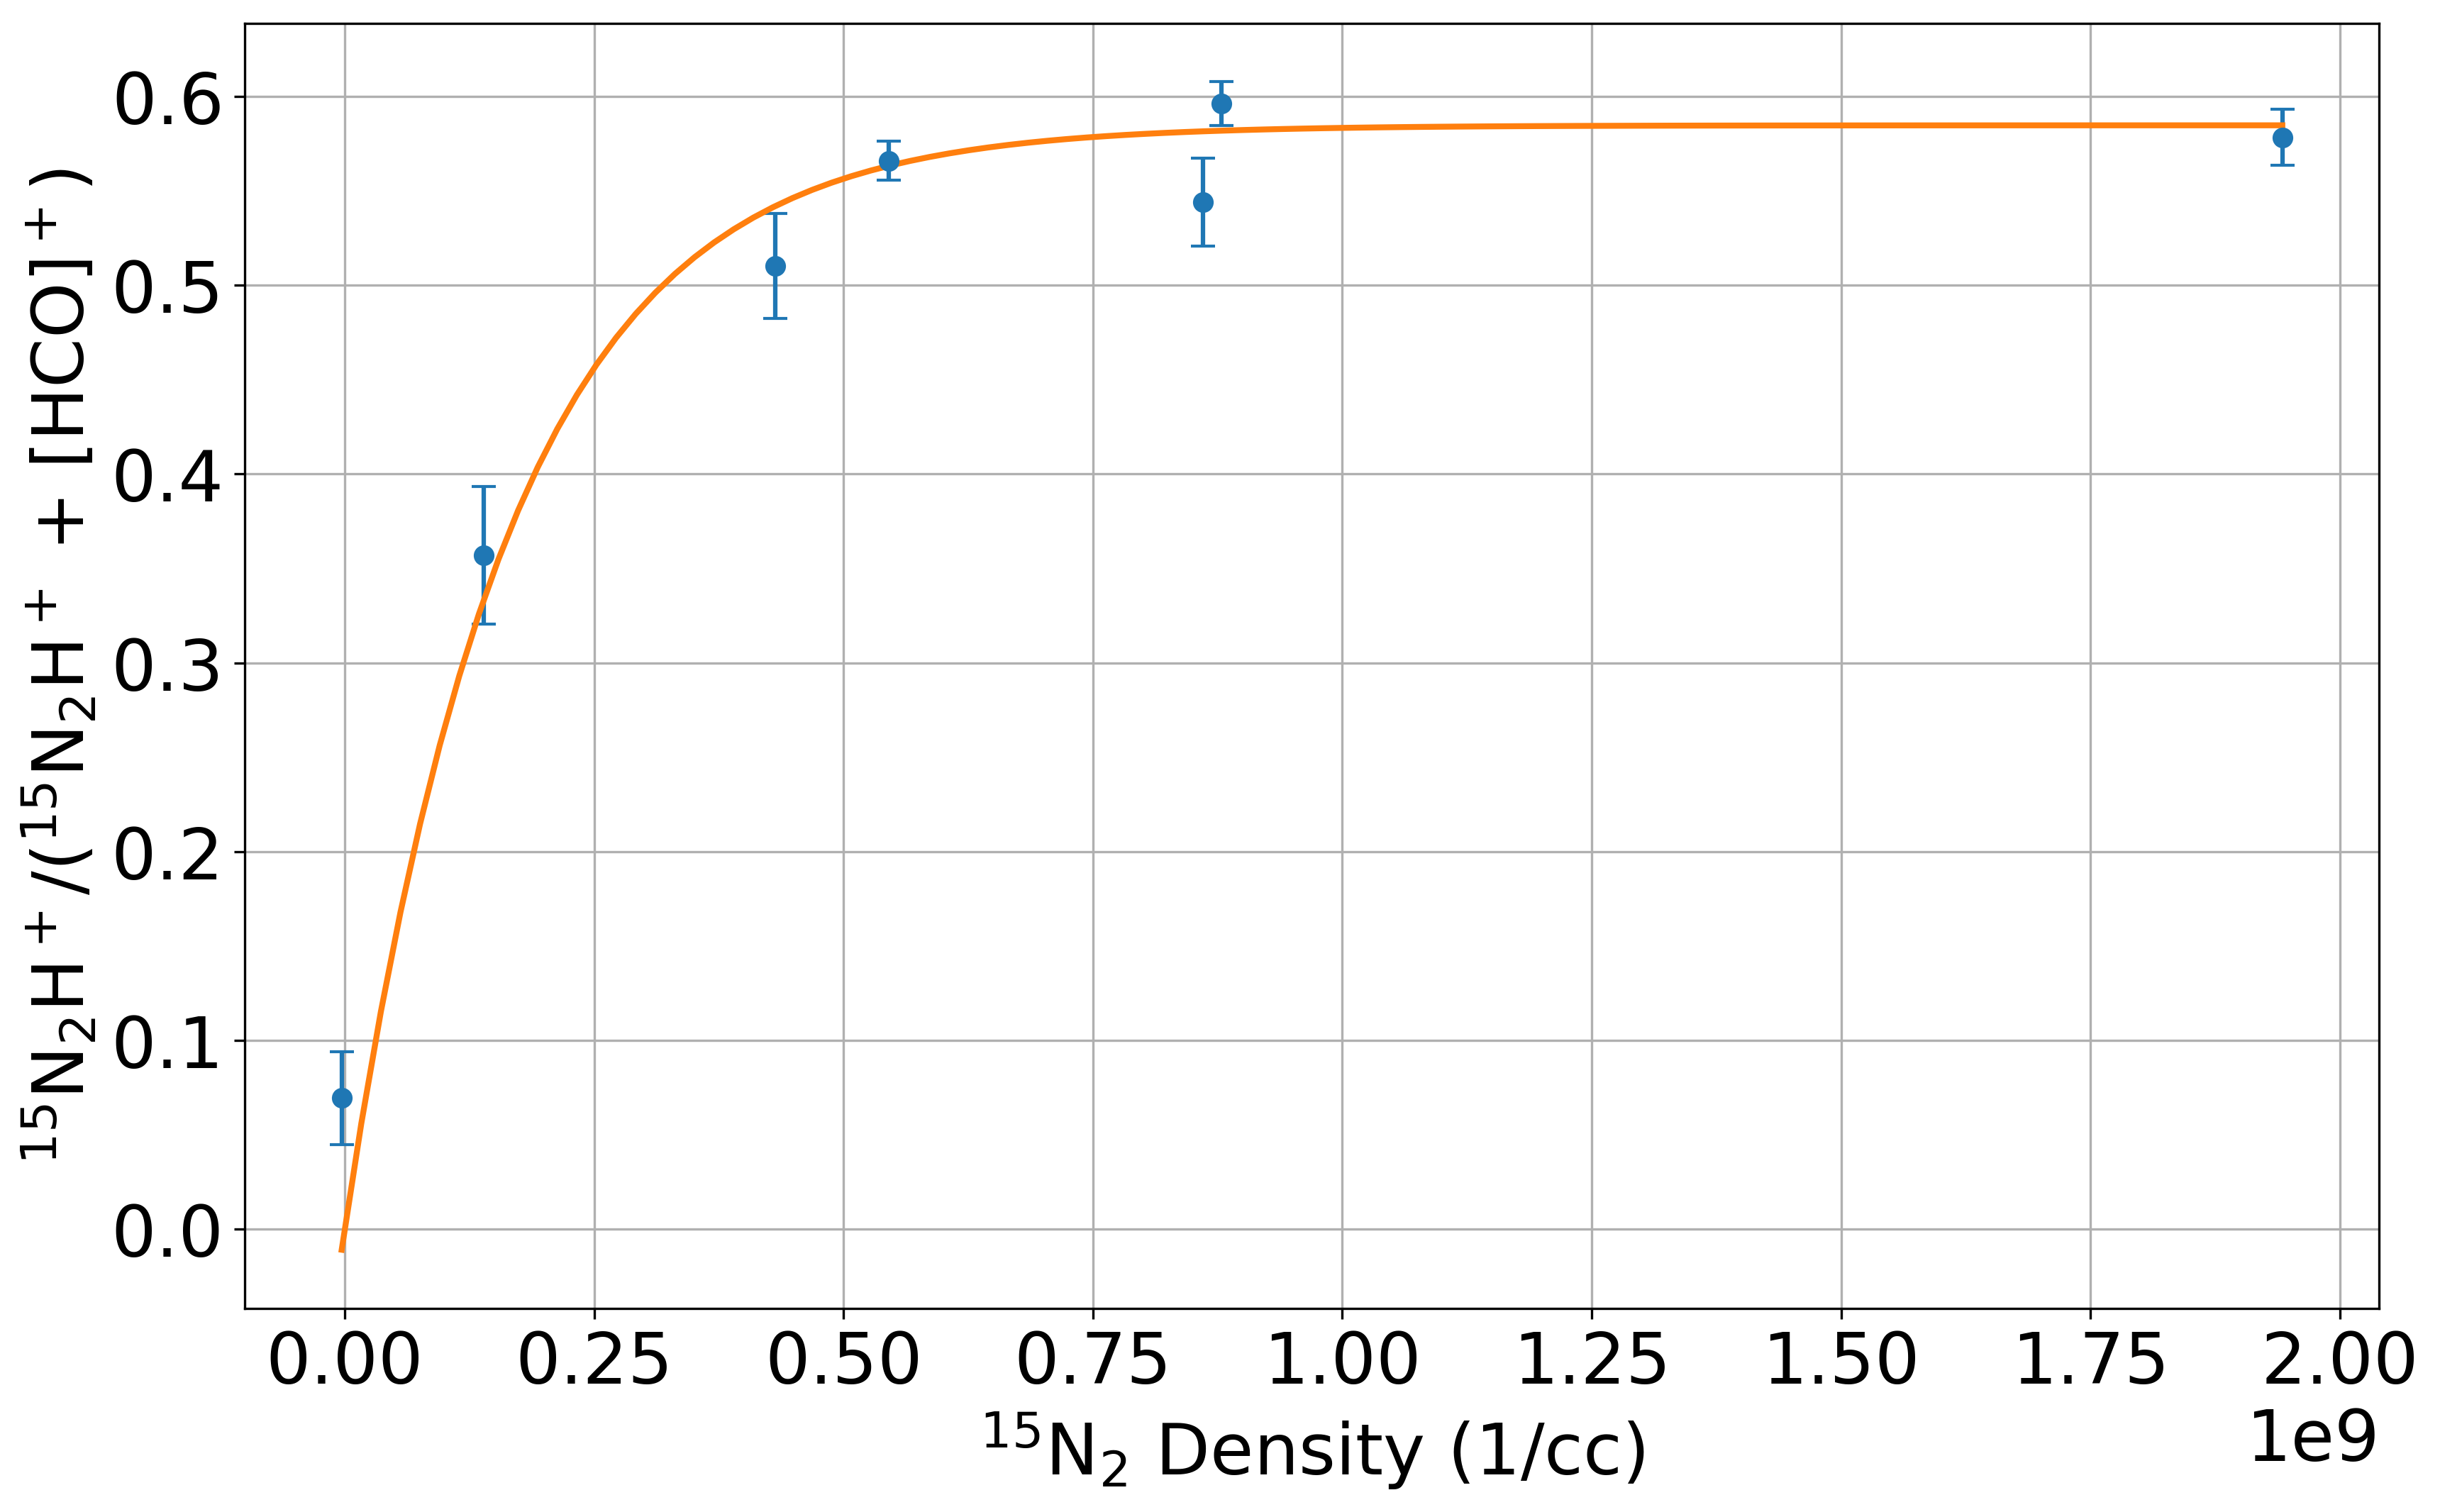
\includegraphics[width=0.8\textwidth]{images/N2_pressure_scan.png}
	\caption{$C = 0.58 \pm 0.02$ $k_{\ref{r: X+COH->XH}} = ((6.1 \pm 1.5) \times 10^{-10})$cm$^3$/s}
\end{figure}